\documentclass{article}
\usepackage{iclr2027_conference,times}
\renewcommand{\ttdefault}{cmtt}
%%%%% NEW MATH DEFINITIONS %%%%%

\usepackage{amsmath,amsfonts,bm}

% Mark sections of captions for referring to divisions of figures
\newcommand{\figleft}{{\em (Left)}}
\newcommand{\figcenter}{{\em (Center)}}
\newcommand{\figright}{{\em (Right)}}
\newcommand{\figtop}{{\em (Top)}}
\newcommand{\figbottom}{{\em (Bottom)}}
\newcommand{\captiona}{{\em (a)}}
\newcommand{\captionb}{{\em (b)}}
\newcommand{\captionc}{{\em (c)}}
\newcommand{\captiond}{{\em (d)}}

% Highlight a newly defined term
\newcommand{\newterm}[1]{{\bf #1}}


% Figure reference, lower-case.
\def\figref#1{figure~\ref{#1}}
% Figure reference, capital. For start of sentence
\def\Figref#1{Figure~\ref{#1}}
\def\twofigref#1#2{figures \ref{#1} and \ref{#2}}
\def\quadfigref#1#2#3#4{figures \ref{#1}, \ref{#2}, \ref{#3} and \ref{#4}}
% Section reference, lower-case.
\def\secref#1{section~\ref{#1}}
% Section reference, capital.
\def\Secref#1{Section~\ref{#1}}
% Reference to two sections.
\def\twosecrefs#1#2{sections \ref{#1} and \ref{#2}}
% Reference to three sections.
\def\secrefs#1#2#3{sections \ref{#1}, \ref{#2} and \ref{#3}}
% Reference to an equation, lower-case.
\def\eqref#1{equation~\ref{#1}}
% Reference to an equation, upper case
\def\Eqref#1{Equation~\ref{#1}}
% A raw reference to an equation---avoid using if possible
\def\plaineqref#1{\ref{#1}}
% Reference to a chapter, lower-case.
\def\chapref#1{chapter~\ref{#1}}
% Reference to an equation, upper case.
\def\Chapref#1{Chapter~\ref{#1}}
% Reference to a range of chapters
\def\rangechapref#1#2{chapters\ref{#1}--\ref{#2}}
% Reference to an algorithm, lower-case.
\def\algref#1{algorithm~\ref{#1}}
% Reference to an algorithm, upper case.
\def\Algref#1{Algorithm~\ref{#1}}
\def\twoalgref#1#2{algorithms \ref{#1} and \ref{#2}}
\def\Twoalgref#1#2{Algorithms \ref{#1} and \ref{#2}}
% Reference to a part, lower case
\def\partref#1{part~\ref{#1}}
% Reference to a part, upper case
\def\Partref#1{Part~\ref{#1}}
\def\twopartref#1#2{parts \ref{#1} and \ref{#2}}

\def\ceil#1{\lceil #1 \rceil}
\def\floor#1{\lfloor #1 \rfloor}
\def\1{\bm{1}}
\newcommand{\train}{\mathcal{D}}
\newcommand{\valid}{\mathcal{D_{\mathrm{valid}}}}
\newcommand{\test}{\mathcal{D_{\mathrm{test}}}}

\def\eps{{\epsilon}}


% Random variables
\def\reta{{\textnormal{$\eta$}}}
\def\ra{{\textnormal{a}}}
\def\rb{{\textnormal{b}}}
\def\rc{{\textnormal{c}}}
\def\rd{{\textnormal{d}}}
\def\re{{\textnormal{e}}}
\def\rf{{\textnormal{f}}}
\def\rg{{\textnormal{g}}}
\def\rh{{\textnormal{h}}}
\def\ri{{\textnormal{i}}}
\def\rj{{\textnormal{j}}}
\def\rk{{\textnormal{k}}}
\def\rl{{\textnormal{l}}}
% rm is already a command, just don't name any random variables m
\def\rn{{\textnormal{n}}}
\def\ro{{\textnormal{o}}}
\def\rp{{\textnormal{p}}}
\def\rq{{\textnormal{q}}}
\def\rr{{\textnormal{r}}}
\def\rs{{\textnormal{s}}}
\def\rt{{\textnormal{t}}}
\def\ru{{\textnormal{u}}}
\def\rv{{\textnormal{v}}}
\def\rw{{\textnormal{w}}}
\def\rx{{\textnormal{x}}}
\def\ry{{\textnormal{y}}}
\def\rz{{\textnormal{z}}}

% Random vectors
\def\rvepsilon{{\mathbf{\epsilon}}}
\def\rvtheta{{\mathbf{\theta}}}
\def\rva{{\mathbf{a}}}
\def\rvb{{\mathbf{b}}}
\def\rvc{{\mathbf{c}}}
\def\rvd{{\mathbf{d}}}
\def\rve{{\mathbf{e}}}
\def\rvf{{\mathbf{f}}}
\def\rvg{{\mathbf{g}}}
\def\rvh{{\mathbf{h}}}
\def\rvu{{\mathbf{i}}}
\def\rvj{{\mathbf{j}}}
\def\rvk{{\mathbf{k}}}
\def\rvl{{\mathbf{l}}}
\def\rvm{{\mathbf{m}}}
\def\rvn{{\mathbf{n}}}
\def\rvo{{\mathbf{o}}}
\def\rvp{{\mathbf{p}}}
\def\rvq{{\mathbf{q}}}
\def\rvr{{\mathbf{r}}}
\def\rvs{{\mathbf{s}}}
\def\rvt{{\mathbf{t}}}
\def\rvu{{\mathbf{u}}}
\def\rvv{{\mathbf{v}}}
\def\rvw{{\mathbf{w}}}
\def\rvx{{\mathbf{x}}}
\def\rvy{{\mathbf{y}}}
\def\rvz{{\mathbf{z}}}

% Elements of random vectors
\def\erva{{\textnormal{a}}}
\def\ervb{{\textnormal{b}}}
\def\ervc{{\textnormal{c}}}
\def\ervd{{\textnormal{d}}}
\def\erve{{\textnormal{e}}}
\def\ervf{{\textnormal{f}}}
\def\ervg{{\textnormal{g}}}
\def\ervh{{\textnormal{h}}}
\def\ervi{{\textnormal{i}}}
\def\ervj{{\textnormal{j}}}
\def\ervk{{\textnormal{k}}}
\def\ervl{{\textnormal{l}}}
\def\ervm{{\textnormal{m}}}
\def\ervn{{\textnormal{n}}}
\def\ervo{{\textnormal{o}}}
\def\ervp{{\textnormal{p}}}
\def\ervq{{\textnormal{q}}}
\def\ervr{{\textnormal{r}}}
\def\ervs{{\textnormal{s}}}
\def\ervt{{\textnormal{t}}}
\def\ervu{{\textnormal{u}}}
\def\ervv{{\textnormal{v}}}
\def\ervw{{\textnormal{w}}}
\def\ervx{{\textnormal{x}}}
\def\ervy{{\textnormal{y}}}
\def\ervz{{\textnormal{z}}}

% Random matrices
\def\rmA{{\mathbf{A}}}
\def\rmB{{\mathbf{B}}}
\def\rmC{{\mathbf{C}}}
\def\rmD{{\mathbf{D}}}
\def\rmE{{\mathbf{E}}}
\def\rmF{{\mathbf{F}}}
\def\rmG{{\mathbf{G}}}
\def\rmH{{\mathbf{H}}}
\def\rmI{{\mathbf{I}}}
\def\rmJ{{\mathbf{J}}}
\def\rmK{{\mathbf{K}}}
\def\rmL{{\mathbf{L}}}
\def\rmM{{\mathbf{M}}}
\def\rmN{{\mathbf{N}}}
\def\rmO{{\mathbf{O}}}
\def\rmP{{\mathbf{P}}}
\def\rmQ{{\mathbf{Q}}}
\def\rmR{{\mathbf{R}}}
\def\rmS{{\mathbf{S}}}
\def\rmT{{\mathbf{T}}}
\def\rmU{{\mathbf{U}}}
\def\rmV{{\mathbf{V}}}
\def\rmW{{\mathbf{W}}}
\def\rmX{{\mathbf{X}}}
\def\rmY{{\mathbf{Y}}}
\def\rmZ{{\mathbf{Z}}}

% Elements of random matrices
\def\ermA{{\textnormal{A}}}
\def\ermB{{\textnormal{B}}}
\def\ermC{{\textnormal{C}}}
\def\ermD{{\textnormal{D}}}
\def\ermE{{\textnormal{E}}}
\def\ermF{{\textnormal{F}}}
\def\ermG{{\textnormal{G}}}
\def\ermH{{\textnormal{H}}}
\def\ermI{{\textnormal{I}}}
\def\ermJ{{\textnormal{J}}}
\def\ermK{{\textnormal{K}}}
\def\ermL{{\textnormal{L}}}
\def\ermM{{\textnormal{M}}}
\def\ermN{{\textnormal{N}}}
\def\ermO{{\textnormal{O}}}
\def\ermP{{\textnormal{P}}}
\def\ermQ{{\textnormal{Q}}}
\def\ermR{{\textnormal{R}}}
\def\ermS{{\textnormal{S}}}
\def\ermT{{\textnormal{T}}}
\def\ermU{{\textnormal{U}}}
\def\ermV{{\textnormal{V}}}
\def\ermW{{\textnormal{W}}}
\def\ermX{{\textnormal{X}}}
\def\ermY{{\textnormal{Y}}}
\def\ermZ{{\textnormal{Z}}}

% Vectors
\def\vzero{{\bm{0}}}
\def\vone{{\bm{1}}}
\def\vmu{{\bm{\mu}}}
\def\vtheta{{\bm{\theta}}}
\def\va{{\bm{a}}}
\def\vb{{\bm{b}}}
\def\vc{{\bm{c}}}
\def\vd{{\bm{d}}}
\def\ve{{\bm{e}}}
\def\vf{{\bm{f}}}
\def\vg{{\bm{g}}}
\def\vh{{\bm{h}}}
\def\vi{{\bm{i}}}
\def\vj{{\bm{j}}}
\def\vk{{\bm{k}}}
\def\vl{{\bm{l}}}
\def\vm{{\bm{m}}}
\def\vn{{\bm{n}}}
\def\vo{{\bm{o}}}
\def\vp{{\bm{p}}}
\def\vq{{\bm{q}}}
\def\vr{{\bm{r}}}
\def\vs{{\bm{s}}}
\def\vt{{\bm{t}}}
\def\vu{{\bm{u}}}
\def\vv{{\bm{v}}}
\def\vw{{\bm{w}}}
\def\vx{{\bm{x}}}
\def\vy{{\bm{y}}}
\def\vz{{\bm{z}}}

% Elements of vectors
\def\evalpha{{\alpha}}
\def\evbeta{{\beta}}
\def\evepsilon{{\epsilon}}
\def\evlambda{{\lambda}}
\def\evomega{{\omega}}
\def\evmu{{\mu}}
\def\evpsi{{\psi}}
\def\evsigma{{\sigma}}
\def\evtheta{{\theta}}
\def\eva{{a}}
\def\evb{{b}}
\def\evc{{c}}
\def\evd{{d}}
\def\eve{{e}}
\def\evf{{f}}
\def\evg{{g}}
\def\evh{{h}}
\def\evi{{i}}
\def\evj{{j}}
\def\evk{{k}}
\def\evl{{l}}
\def\evm{{m}}
\def\evn{{n}}
\def\evo{{o}}
\def\evp{{p}}
\def\evq{{q}}
\def\evr{{r}}
\def\evs{{s}}
\def\evt{{t}}
\def\evu{{u}}
\def\evv{{v}}
\def\evw{{w}}
\def\evx{{x}}
\def\evy{{y}}
\def\evz{{z}}

% Matrix
\def\mA{{\bm{A}}}
\def\mB{{\bm{B}}}
\def\mC{{\bm{C}}}
\def\mD{{\bm{D}}}
\def\mE{{\bm{E}}}
\def\mF{{\bm{F}}}
\def\mG{{\bm{G}}}
\def\mH{{\bm{H}}}
\def\mI{{\bm{I}}}
\def\mJ{{\bm{J}}}
\def\mK{{\bm{K}}}
\def\mL{{\bm{L}}}
\def\mM{{\bm{M}}}
\def\mN{{\bm{N}}}
\def\mO{{\bm{O}}}
\def\mP{{\bm{P}}}
\def\mQ{{\bm{Q}}}
\def\mR{{\bm{R}}}
\def\mS{{\bm{S}}}
\def\mT{{\bm{T}}}
\def\mU{{\bm{U}}}
\def\mV{{\bm{V}}}
\def\mW{{\bm{W}}}
\def\mX{{\bm{X}}}
\def\mY{{\bm{Y}}}
\def\mZ{{\bm{Z}}}
\def\mBeta{{\bm{\beta}}}
\def\mPhi{{\bm{\Phi}}}
\def\mLambda{{\bm{\Lambda}}}
\def\mSigma{{\bm{\Sigma}}}

% Tensor
\DeclareMathAlphabet{\mathsfit}{\encodingdefault}{\sfdefault}{m}{sl}
\SetMathAlphabet{\mathsfit}{bold}{\encodingdefault}{\sfdefault}{bx}{n}
\newcommand{\tens}[1]{\bm{\mathsfit{#1}}}
\def\tA{{\tens{A}}}
\def\tB{{\tens{B}}}
\def\tC{{\tens{C}}}
\def\tD{{\tens{D}}}
\def\tE{{\tens{E}}}
\def\tF{{\tens{F}}}
\def\tG{{\tens{G}}}
\def\tH{{\tens{H}}}
\def\tI{{\tens{I}}}
\def\tJ{{\tens{J}}}
\def\tK{{\tens{K}}}
\def\tL{{\tens{L}}}
\def\tM{{\tens{M}}}
\def\tN{{\tens{N}}}
\def\tO{{\tens{O}}}
\def\tP{{\tens{P}}}
\def\tQ{{\tens{Q}}}
\def\tR{{\tens{R}}}
\def\tS{{\tens{S}}}
\def\tT{{\tens{T}}}
\def\tU{{\tens{U}}}
\def\tV{{\tens{V}}}
\def\tW{{\tens{W}}}
\def\tX{{\tens{X}}}
\def\tY{{\tens{Y}}}
\def\tZ{{\tens{Z}}}


% Graph
\def\gA{{\mathcal{A}}}
\def\gB{{\mathcal{B}}}
\def\gC{{\mathcal{C}}}
\def\gD{{\mathcal{D}}}
\def\gE{{\mathcal{E}}}
\def\gF{{\mathcal{F}}}
\def\gG{{\mathcal{G}}}
\def\gH{{\mathcal{H}}}
\def\gI{{\mathcal{I}}}
\def\gJ{{\mathcal{J}}}
\def\gK{{\mathcal{K}}}
\def\gL{{\mathcal{L}}}
\def\gM{{\mathcal{M}}}
\def\gN{{\mathcal{N}}}
\def\gO{{\mathcal{O}}}
\def\gP{{\mathcal{P}}}
\def\gQ{{\mathcal{Q}}}
\def\gR{{\mathcal{R}}}
\def\gS{{\mathcal{S}}}
\def\gT{{\mathcal{T}}}
\def\gU{{\mathcal{U}}}
\def\gV{{\mathcal{V}}}
\def\gW{{\mathcal{W}}}
\def\gX{{\mathcal{X}}}
\def\gY{{\mathcal{Y}}}
\def\gZ{{\mathcal{Z}}}

% Sets
\def\sA{{\mathbb{A}}}
\def\sB{{\mathbb{B}}}
\def\sC{{\mathbb{C}}}
\def\sD{{\mathbb{D}}}
% Don't use a set called E, because this would be the same as our symbol
% for expectation.
\def\sF{{\mathbb{F}}}
\def\sG{{\mathbb{G}}}
\def\sH{{\mathbb{H}}}
\def\sI{{\mathbb{I}}}
\def\sJ{{\mathbb{J}}}
\def\sK{{\mathbb{K}}}
\def\sL{{\mathbb{L}}}
\def\sM{{\mathbb{M}}}
\def\sN{{\mathbb{N}}}
\def\sO{{\mathbb{O}}}
\def\sP{{\mathbb{P}}}
\def\sQ{{\mathbb{Q}}}
\def\sR{{\mathbb{R}}}
\def\sS{{\mathbb{S}}}
\def\sT{{\mathbb{T}}}
\def\sU{{\mathbb{U}}}
\def\sV{{\mathbb{V}}}
\def\sW{{\mathbb{W}}}
\def\sX{{\mathbb{X}}}
\def\sY{{\mathbb{Y}}}
\def\sZ{{\mathbb{Z}}}

% Entries of a matrix
\def\emLambda{{\Lambda}}
\def\emA{{A}}
\def\emB{{B}}
\def\emC{{C}}
\def\emD{{D}}
\def\emE{{E}}
\def\emF{{F}}
\def\emG{{G}}
\def\emH{{H}}
\def\emI{{I}}
\def\emJ{{J}}
\def\emK{{K}}
\def\emL{{L}}
\def\emM{{M}}
\def\emN{{N}}
\def\emO{{O}}
\def\emP{{P}}
\def\emQ{{Q}}
\def\emR{{R}}
\def\emS{{S}}
\def\emT{{T}}
\def\emU{{U}}
\def\emV{{V}}
\def\emW{{W}}
\def\emX{{X}}
\def\emY{{Y}}
\def\emZ{{Z}}
\def\emSigma{{\Sigma}}

% entries of a tensor
% Same font as tensor, without \bm wrapper
\newcommand{\etens}[1]{\mathsfit{#1}}
\def\etLambda{{\etens{\Lambda}}}
\def\etA{{\etens{A}}}
\def\etB{{\etens{B}}}
\def\etC{{\etens{C}}}
\def\etD{{\etens{D}}}
\def\etE{{\etens{E}}}
\def\etF{{\etens{F}}}
\def\etG{{\etens{G}}}
\def\etH{{\etens{H}}}
\def\etI{{\etens{I}}}
\def\etJ{{\etens{J}}}
\def\etK{{\etens{K}}}
\def\etL{{\etens{L}}}
\def\etM{{\etens{M}}}
\def\etN{{\etens{N}}}
\def\etO{{\etens{O}}}
\def\etP{{\etens{P}}}
\def\etQ{{\etens{Q}}}
\def\etR{{\etens{R}}}
\def\etS{{\etens{S}}}
\def\etT{{\etens{T}}}
\def\etU{{\etens{U}}}
\def\etV{{\etens{V}}}
\def\etW{{\etens{W}}}
\def\etX{{\etens{X}}}
\def\etY{{\etens{Y}}}
\def\etZ{{\etens{Z}}}

% The true underlying data generating distribution
\newcommand{\pdata}{p_{\rm{data}}}
% The empirical distribution defined by the training set
\newcommand{\ptrain}{\hat{p}_{\rm{data}}}
\newcommand{\Ptrain}{\hat{P}_{\rm{data}}}
% The model distribution
\newcommand{\pmodel}{p_{\rm{model}}}
\newcommand{\Pmodel}{P_{\rm{model}}}
\newcommand{\ptildemodel}{\tilde{p}_{\rm{model}}}
% Stochastic autoencoder distributions
\newcommand{\pencode}{p_{\rm{encoder}}}
\newcommand{\pdecode}{p_{\rm{decoder}}}
\newcommand{\precons}{p_{\rm{reconstruct}}}

\newcommand{\laplace}{\mathrm{Laplace}} % Laplace distribution

\newcommand{\E}{\mathbb{E}}
\newcommand{\Ls}{\mathcal{L}}
\newcommand{\R}{\mathbb{R}}
\newcommand{\emp}{\tilde{p}}
\newcommand{\lr}{\alpha}
\newcommand{\reg}{\lambda}
\newcommand{\rect}{\mathrm{rectifier}}
\newcommand{\softmax}{\mathrm{softmax}}
\newcommand{\sigmoid}{\sigma}
\newcommand{\softplus}{\zeta}
\newcommand{\KL}{D_{\mathrm{KL}}}
\newcommand{\Var}{\mathrm{Var}}
\newcommand{\standarderror}{\mathrm{SE}}
\newcommand{\Cov}{\mathrm{Cov}}
% Wolfram Mathworld says $L^2$ is for function spaces and $\ell^2$ is for vectors
% But then they seem to use $L^2$ for vectors throughout the site, and so does
% wikipedia.
\newcommand{\normlzero}{L^0}
\newcommand{\normlone}{L^1}
\newcommand{\normltwo}{L^2}
\newcommand{\normlp}{L^p}
\newcommand{\normmax}{L^\infty}

\newcommand{\parents}{Pa} % See usage in notation.tex. Chosen to match Daphne's book.

\DeclareMathOperator*{\argmax}{arg\,max}
\DeclareMathOperator*{\argmin}{arg\,min}

\DeclareMathOperator{\sign}{sign}
\DeclareMathOperator{\Tr}{Tr}
\let\ab\allowbreak


\usepackage{hyperref}
\usepackage{url}
\usepackage{booktabs}
\usepackage{tabularx}
\usepackage{array}
\usepackage{graphicx}
\usepackage{float}
\usepackage{subcaption}
\usepackage{amsmath,amssymb,amsfonts,amsthm}
\usepackage{bm}
\usepackage{xcolor}
\usepackage{listings}

\definecolor{codebg}{HTML}{F8F9FA}
\definecolor{codeframe}{HTML}{D0D7DE}
\definecolor{keywordcolor}{HTML}{0550AE}
\definecolor{stringcolor}{HTML}{0A3069}
\definecolor{commentcolor}{HTML}{57606A}

\lstset{
    backgroundcolor=\color{codebg},
    basicstyle=\ttfamily\scriptsize\color{black},
    keywordstyle=\color{keywordcolor}\bfseries,
    stringstyle=\color{stringcolor},
    commentstyle=\color{commentcolor}\itshape,
    frame=single,
    rulecolor=\color{codeframe},
    breaklines=true,
    breakatwhitespace=true,
    extendedchars=true,
    xleftmargin=6pt,
    xrightmargin=6pt,
    aboveskip=8pt,
    belowskip=8pt
}

\hypersetup{
    colorlinks=true,
    linkcolor=blue!70!black,
    citecolor=blue!70!black,
    urlcolor=blue!70!black
}

\title{\textbf{PHANTOM: Parameter-Hashed Attention with Token-wise Orthogonal Mapping}

\author{Anonymous authors}


\newcommand{\fix}{\marginpar{FIX}}
\newcommand{\new}{\marginpar{NEW}}

\begin{document}

\maketitle

\begin{abstract}
Standard transformer attention couples two independent problems: how to 
project hidden states into query/key/value representations (a **dense linear 
algebra** problem), and how to compute the attention weights themselves (a 
\textbf{quadratic matching} problem). We introduce \textbf{PHANTOM} 
(\textbf{P}arameter-\textbf{H}ashed \textbf{A}ttentio\textbf{N} with \textbf{T}oken-wise 
\textbf{O}rthogonal \textbf{M}apping), which addresses both problems with a unified 
architecture. Projections are compressed via **leverage-score CUR matrix 
decomposition**, replacing each $W \in \mathbb{R}^{d_\text{out} \times d_\text{in}}$ 
with a low-rank product $C U^+ R$ that preserves statistically important rows 
and columns. Attention is computed via \textbf{multi-round angular LSH}, which 
partitions tokens into hash buckets by random projection signs and computes 
attention only within buckets, reducing effective cost from $\mathcal{O}(L^2)$ 
to $\mathcal{O}(L \cdot B)$ where $B$ is the average bucket size. We use a 
\textbf{rectified softpick} activation instead of softmax, which drops far-tail 
attention weights while falling back to softmax when no candidate survives.

PHANTOM compresses DistilBERT by \textbf{50\%$$\times$}, RoBERTa by \textbf{2.1$$\times$}, 
and GPT-2 by \textbf{2.1$$\times$}, with SST-2 accuracy drops of only 
\textbf{-18.12\%}, \textbf{-27.64\%}, and \textbf{-28.44\%} after 
50 LoRA recovery steps. Peak inference VRAM decreases by 
\textbf{380 MB\%}. Unlike attention-replacement methods that preserve 
parameter count, PHANTOM achieves genuine parameter reduction from 
$d_\text{in} d_\text{out}$ to $r(d_\text{in} + d_\text{out})$ via CUR 
factorization. We provide a production-hardened implementation with strict 
Frobenius validation, safe per-layer fallback, and multi-architecture support.

\textbf{Keywords:} CUR decomposition, leverage scores, locality-sensitive hashing, 
sparse attention, transformer compression, softpick



\vspace{0.5em}
\noindent\textbf{Keywords:} CUR decomposition, leverage scores, locality-sensitive hashing,
\end{abstract}

\section{01 Intro}

Draft content for phantom.


\section{Related Work}

\subsection{Low-Rank Matrix Decomposition}

\subsubsection{SVD and Eckart--Young}

The truncated SVD is optimal in Frobenius norm (Eckart \& Young, 1936). However, 
the factors $U, V$ are dense and orthogonal, which limits interpretability.

\subsubsection{CUR Decomposition}

Mahoney \& Drineas (2009) introduced CUR as an interpretable alternative: 
select $r$ columns and $r$ rows of $W$, then reconstruct as $C \cdot U^+ \cdot R$ 
where $U$ is the intersection. The key insight is that **statistical leverage 
scores** (Mahoney et al., 2012) provide the optimal sampling probabilities. 
PHANTOM uses deterministic top-$r$ selection by leverage score.

\subsubsection{Randomized SVD}

Halko et al. (2011) provide randomized SVD with complexity 
$\mathcal{O}(d^2 r)$. We use exact SVD for leverage computation because 
matrix sizes are manageable.

\subsection{Sparse Attention}

\subsubsection{Fixed-Pattern Sparsity}

Longformer (Beltagy et al., 2020) uses a sliding window plus global tokens. 
BigBird (Zaheer et al., 2020) adds random edges. Both use \textbf{fixed} patterns 
that do not adapt to input.

\subsubsection{Content-Based Sparsity}

Reformer (Kitaev et al., 2020) uses LSH to group similar queries and keys. 
Routing Transformer (Roy et al., 2021) uses online k-means. PHANTOM uses 
\textbf{multi-round angular LSH} with a rectangular hash function that is 
differentiable through sign operations.

\subsubsection{Comparisons}

\begin{table}[H]
\centering
\small
\begin{tabular}{llll}
\toprule
\textbf{Method} & \textbf{Pattern} & \textbf{Adaptive} & \textbf{Complexity} \\
\midrule
Longformer & Sliding window + global & No & $\mathcal{O}(L \sqrt{L})$ \\
BigBird & Window + random + global & No & $\mathcal{O}(L)$ \\
Reformer & LSH buckets & Yes & $\mathcal{O}(L \log L)$ \\
Routing & k-means clusters & Yes & $\mathcal{O}(L \log L)$ \\
\textbf{PHANTOM} & Multi-round angular LSH & Yes & $\mathcal{O}(L \cdot B)$ \\
\bottomrule
\end{tabular}
\end{table}

\subsection{Attention Activations}

\subsubsection{Softmax}

Standard softmax has two limitations: (i) it never reaches exactly zero, so 
far-tail positions receive non-negligible weight; (ii) it is sensitive to 
outliers.

\subsubsection{Sparsemax}

Martins \& Astudillo (2016) propose sparsemax, which projects onto the simplex 
and produces sparse attention. However, sparsemax has no closed-form for 
batched computation.

\subsubsection{Softpick}

Lu et al. (2024) propose softpick: $\text{ReLU}(e^{(x_i - m)} - e^{-m})$ 
where $m = \max_j x_j$. This is sparse and has closed form. We use a 
\textbf{rectified} variant with a softmax fallback when the denominator is zero.

\subsection{Post-Training Compression}

\begin{table}[H]
\centering
\small
\begin{tabular}{lllll}
\toprule
\textbf{Method} & \textbf{Type} & \textbf{Retrain?} & \textbf{Compression} & \textbf{Attention?} \\
\midrule
SVD (Eckart-Young) & Low-rank & No & Ratio $r$ & No \\
A3 & Fisher-weighted SVD & LoRA & Ratio $r$ & No \\
AASVD & Covariance-weighted SVD & LoRA & Ratio $r$ & No \\
SparseGPT & Pruning & No & 50\% & No \\
\textbf{PHANTOM} & CUR + LSH & LoRA & Ratio $r$ & \textbf{Yes} \\
\bottomrule
\end{tabular}
\end{table}

\textbf{Key distinction.} PHANTOM is the only method in this list that compresses 
both \textbf{projections} (via CUR) \textbf{and attention} (via LSH).

\subsection{Position of Our Work}

PHANTOM is unique in combining:
\begin{enumerate}
\item \textbf{CUR decomposition} for interpretable low-rank projections.
\item \textbf{Multi-round LSH} for content-adaptive sparse attention.
\item \textbf{Rectified softpick} for stable sparse attention.

\end{enumerate}
Prior work addresses each of these individually, but no prior method combines 
all three.
\begin{lstlisting}

---
\end{lstlisting}

\section{Background}

\subsection{The CUR Decomposition}

For a matrix $W \in \mathbb{R}^{m \times n}$ and target rank $r$, CUR selects:

\[
W \approx C \cdot U^+ \cdot R
\tag{3.1}
\]

where:
\begin{itemize}
\item $C \in \mathbb{R}^{m \times r}$ contains $r$ columns of $W$.
\item $R \in \mathbb{R}^{r \times n}$ contains $r$ rows of $W$.
\item $U \in \mathbb{R}^{r \times r}$ is the intersection matrix $W[\text{rows}, \text{cols}]$.
\item $U^+$ is the Moore--Penrose pseudoinverse.

\end{itemize}
\textbf{Error bound.} Drineas et al. (2008) prove that if columns and rows are 
sampled with probability proportional to leverage scores, then:

\[
\|W - C U^+ R\|_F \leq (1 + \epsilon) \|W - W_r\|_F
\tag{3.2}
\]

with probability $1 - \delta$ for sample size 
$r = \mathcal{O}(r^* / \epsilon^2 \log(1/\delta))$.

\subsection{Leverage Scores}

For a matrix $W = U \Sigma V^\top$ with rank $r^*$, the \textbf{column leverage score} 
of column $j$ is:

\[
\pi_j = \sum_{k=1}^{r^*} (V_{j, k})^2
\tag{3.3}
\]

and the \textbf{row leverage score} of row $i$ is:

\[
\rho_i = \sum_{k=1}^{r^*} (U_{i, k})^2
\tag{3.4}
\]

Leverage scores satisfy $\sum_j \pi_j = r^\textit{$ and $\sum_i \rho_i = r^}$. The 
scores measure how important each row/column is for the low-rank structure 
of $W$.

\textbf{Deterministic top-$r$ selection.} Instead of sampling, PHANTOM selects 
the $r$ rows/columns with highest leverage. This is deterministic and gives 
the best rank-$r$ CUR approximation in practice.

\subsection{Angular LSH}

Angular LSH (Charikar, 2002) hashes vectors based on their direction. For a 
random projection $a \sim \mathcal{N}(0, I_d)$, define:

\[
h_a(x) = \text{sign}(a^\top x) \in \{-1, +1\}
\tag{3.5}
\]

For $k$ independent projections $a_1, \dots, a_k$, the $k$-bit hash is:

\[
H(x) = \sum_{i=1}^{k} 2^{i-1} \cdot \mathbb{1}[h_{a_i}(x) = +1]
\tag{3.6}
\]

\textbf{Collision probability.} For two vectors $x, y$ with angle $\theta$ between 
them:

\[
\Pr[H(x) = H(y)] = 1 - \frac{\theta}{\pi}
\tag{3.7}
\]

so vectors with small angles collide with high probability.

\textbf{Multi-round LSH.} A single LSH round has high variance. PHANTOM applies 
$R_\ell$ independent rounds, each with a fresh projection matrix, and 
averages the resulting attention outputs:

\[
\text{Output} = \frac{1}{R_\ell} \sum_{r=1}^{R_\ell} \text{Attn}_{\text{LSH}}^{(r)}(Q, K, V)
\tag{3.8}
\]

\subsection{Softpick Activation}

Softpick (Lu et al., 2024) generalizes softmax by subtracting a fixed baseline:

\[
\text{softpick}(x_i) = \text{ReLU}\!\left(e^{(x_i - m)/\tau_s} - e^{-m/\tau_s}\right)
\tag{3.9}
\]

where $m = \max_j x_j$ and $\tau_s$ is a temperature. Positions with 
$x_i \ll m$ are truncated to zero, producing sparse attention.

\textbf{Normalization.} The unnormalized weights are normalized:

\[
\hat{p}_i = \frac{\text{softpick}(x_i)}{\sum_j \text{softpick}(x_j) + \epsilon}
\tag{3.10}
\]

\textbf{Numerical issue.} If $m < 0$ (all attention scores negative, e.g., from 
masking), then $e^{-m/\tau_s} \geq 1$ and the ReLU may zero out the entire 
row. PHANTOM adds a softmax fallback:

\[
p_i = \begin{cases} \hat{p}_i & \text{if } \sum_j \text{softpick}(x_j) > 10^{-5} \\ \text{softmax}(x_i / \tau_s) & \text{otherwise} \end{cases}
\tag{3.11}
\]

\subsection{LoRA Recovery}

LoRA (Hu et al., 2021) adds trainable low-rank adapters to frozen base weights:

\[
W_\text{eff} = W_\text{frozen} + \frac{\alpha}{r_L} B A
\tag{3.12}
\]

PHANTOM uses LoRA on top of the CUR-factorized projections for recovery 
fine-tuning.

\subsection{Notation Summary}

\begin{lstlisting}

---
\end{lstlisting}

\section{Method}

\subsection{Overview}

PHANTOM replaces standard transformer attention with a two-stage compression:

\begin{enumerate}
\item \textbf{Projection compression} ( 4.2): replace each $W \in \{W_Q, W_K, W_V, W_O\}$
  with a CUR factorized layer $C U^+ R$.
\item \textbf{Sparse attention} ( 4.3): compute attention via multi-round angular LSH
  with rectified softpick.

\end{enumerate}
\textbf{Figure 4.1} shows the pipeline.

\begin{lstlisting}
   +--------------------------------------------------+
   |  Input: hidden_states $\in$ R^{B$\times$L$\times$d}                |
   +-------------------+------------------------------+
                       |
                        
   +--------------------------------------------------+
   |  Phase 1: CUR Projections                        |
   |  Q = CUR_Q(hidden_states)                        |
   |  K = CUR_K(hidden_states)                        |
   |  V = CUR_V(hidden_states)                        |
   +-------------------+------------------------------+
                       |
                        
   +--------------------------------------------------+
   |  Phase 2: Multi-Round LSH Attention              |
   |  For round r in 1..R:                            |
   |    hash_Q, hash_K $\leftarrow$ random proj + sign           |
   |    match $\leftarrow$ (hash_Q == hash_K)                    |
   |    attn_r $\leftarrow$ softpick(scores   match)             |
   |  Output = mean(attn_r   V)                       |
   +-------------------+------------------------------+
                       |
                        
   +--------------------------------------------------+
   |  Phase 3: Output Projection (CUR_O)              |
   +-------------------+------------------------------+
                       |
                        
   +--------------------------------------------------+
   |  Output: y $\in$ R^{B$\times$L$\times$d}                           |
   +--------------------------------------------------+
\end{lstlisting}

\subsection{Phase 1: CUR Projection Compression}

\subsubsection{The Factorized Layer}

Each projection $W$ is replaced by a two-layer factorization:

\[
y = U_\text{up} \cdot (D_\text{down} \cdot x) + b
\tag{4.1}
\]

where:
\begin{itemize}
\item $D_\text{down} \in \mathbb{R}^{r \times d_\text{in}}$ is the down projection.
\item $U_\text{up} \in \mathbb{R}^{d_\text{out} \times r}$ is the up projection.

\end{itemize}
\textbf{Parameter count:} $r(d_\text{in} + d_\text{out})$ vs $d_\text{in} d_\text{out}$ 
for the original.

For $d_\text{in} = d_\text{out} = 768$ and $r = 16$:

\begin{table}[H]
\centering
\small
\begin{tabular}{lll}
\toprule
\textbf{Config} & \textbf{Params} & \textbf{Ratio} \\
\midrule
Original & 589,824 & 1.0$\times$ \\
PHANTOM (r=16) & 24,576 & \textbf{24$\times$} \\
PHANTOM + LoRA (r=16) & 49,152 & \textbf{12$\times$} \\
\bottomrule
\end{tabular}
\end{table}

\subsubsection{Leverage-Score Selection}

Given a weight matrix $W \in \mathbb{R}^{d_\text{out} \times d_\text{in}}$, 
we compute its SVD:

\[
W = U \Sigma V^\top
\tag{4.2}
\]

\textbf{Column leverage} (importance of each input dimension):

\[
\pi_j = \sum_{k=1}^{\min(m, n)} (V_{j, k})^2
\tag{4.3}
\]

\textbf{Row leverage} (importance of each output dimension):

\[
\rho_i = \sum_{k=1}^{\min(m, n)} (U_{i, k})^2
\tag{4.4}
\]

We normalize both to sum to 1:

\[
\tilde{\pi}_j = \frac{\pi_j}{\sum_{j'} \pi_{j'}}, \qquad
\tilde{\rho}_i = \frac{\rho_i}{\sum_{i'} \rho_{i'}}
\tag{4.5}
\]

Then select the top-$r$ columns and rows:

\[
\mathcal{J} = \text{top}_r(\tilde{\pi}), \qquad
\mathcal{I} = \text{top}_r(\tilde{\rho})
\tag{4.6}
\]

\subsubsection{CUR Reconstruction}

Define:

\[
C = W[:, \mathcal{J}] \in \mathbb{R}^{d_\text{out} \times r}
\tag{4.7}
\]

\[
R = W[\mathcal{I}, :] \in \mathbb{R}^{r \times d_\text{in}}
\tag{4.8}
\]

\[
W_\text{intersection} = W[\mathcal{I}, \mathcal{J}] \in \mathbb{R}^{r \times r}
\tag{4.9}
\]

The reconstruction is:

\[
W_\text{CUR} = C \cdot W_\text{intersection}^+ \cdot R
\tag{4.10}
\]

\subsubsection{Factor Assignment}

We assign the CUR factors to the down/up projections as follows:

\[
D_\text{down} = R \in \mathbb{R}^{r \times d_\text{in}}
\tag{4.11}
\]

\[
U_\text{up} = C \cdot W_\text{intersection}^+ \in \mathbb{R}^{d_\text{out} \times r}
\tag{4.12}
\]

The factorized layer computes:

\[
y = U_\text{up} \cdot (D_\text{down} \cdot x) + b
\tag{4.13}
\]

\subsubsection{Fallback}

If SVD or pseudoinverse fails (e.g., ill-conditioned matrix), we fall back 
to Kaiming initialization. This rarely occurs but ensures robustness.

\subsection{Phase 2: Multi-Round LSH Attention}

\subsubsection{Angular LSH Construction}

For each of $R_\ell$ rounds:

\begin{enumerate}
\item Sample a random projection matrix $A^{(r)} \in \mathbb{R}^{d_h \times k}$.
\item Normalize each column of $A^{(r)}$ to unit norm.
\item Compute hash codes:
  $$
  h\_Q^{(r)} = \sum\_{i=1}^{k} 2^{i-1} \cdot \mathbb{1}\left[\left(Q\_\text{norm} \cdot A^{(r)}\right)\_i > 0\right]
  \tag{4.14}
  $$
  $$
  h\_K^{(r)} = \sum\_{i=1}^{k} 2^{i-1} \cdot \mathbb{1}\left[\left(K\_\text{norm} \cdot A^{(r)}\right)\_i > 0\right]
  \tag{4.15}
  $$
  where $Q_\text{norm}, K_\text{norm}$ are L2-normalized query/key matrices.

\item Compute the boolean match matrix:
  $$
  M^{(r)}\_{ij} = \mathbb{1}[h\_{Q,i}^{(r)} = h\_{K,j}^{(r)}]
  \tag{4.16}
  $$

\item Always add the diagonal (self-attention):
  $$
  M^{(r)} \leftarrow M^{(r)} \lor I
  \tag{4.17}
  $$

\end{enumerate}
\subsubsection{Masking}

For padding and causality:

\[
M^{(r)}_{ij} \leftarrow M^{(r)}_{ij} \land \text{valid}_j \land (\neg \text{causal}_{ij})
\tag{4.18}
\]

where $\text{causal}_{ij} = \mathbb{1}[i < j]$.

\subsubsection{Attention Computation}

For each round, compute the attention scores:

\[
S^{(r)}_{ij} = \frac{Q_i \cdot K_j^\top}{\sqrt{d_h}}
\tag{4.19}
\]

Then mask and apply softpick:

\[
S^{(r)}_{ij} \leftarrow S^{(r)}_{ij} + (M^{(r)}_{ij} - 1) \cdot \infty
\tag{4.20}
\]

\[
\alpha^{(r)} = \text{softpick}(S^{(r)}, \tau_s)
\tag{4.21}
\]

Apply dropout (if training) and compute the round's output:

\[
O^{(r)} = \alpha^{(r)} \cdot V
\tag{4.22}
\]

\subsubsection{Round Averaging}

The final attention output is the mean over rounds:

\[
O = \frac{1}{R_\ell} \sum_{r=1}^{R_\ell} O^{(r)}
\tag{4.23}
\]

\subsubsection{Choice of Hyperparameters}

\begin{table}[H]
\centering
\small
\begin{tabular}{lll}
\toprule
\textbf{Parameter} & \textbf{Default} & \textbf{Rationale} \\
\midrule
$R_\ell$ (rounds) & 4 & Balances variance vs compute \\
$k$ (bits) & 4 & 16 buckets per round \\
$\tau_s$ & 1.0 & Standard softpick temperature \\
\bottomrule
\end{tabular}
\end{table}

With $k = 4$ bits, the number of buckets per round is $2^4 = 16$. The average 
bucket size is roughly $L / 16$, so sparse attention cost is 
$\mathcal{O}(L^2 / 16)$ -- a 16$\times$ reduction.

\subsection{Rectified Softpick}

We define softpick with a fallback to softmax:

\[
\text{softpick}_i(x) = \text{ReLU}\!\left(e^{(x_i - m)/\tau_s} - e^{-m/\tau_s}\right)
\tag{4.24}
\]

where $m = \max_j x_j$. The output is normalized:

\[
\hat{p}_i = \frac{\text{softpick}_i(x)}{\sum_j \text{softpick}_j(x) + \epsilon}
\tag{4.25}
\]

\textbf{Fallback.} If $\sum_j \text{softpick}_j(x) < 10^{-5}$ (all weights zero), 
we substitute:

\[
p_i = \text{softmax}(x_i / \tau_s)
\tag{4.26}
\]

This handles the case where all attention scores are highly negative (from 
masking), which would otherwise produce a zero row.

\subsection{The Full Algorithm}

\textbf{Algorithm 1:} PHANTOM forward pass
\begin{lstlisting}
Input:  hidden_states $\in$ R^{B$\times$L$\times$d}, mask
Output: y $\in$ R^{B$\times$L$\times$d}

1:  # Phase 1: CUR projections
2:  Q $\leftarrow$ CUR_q(hidden_states)
3:  K $\leftarrow$ CUR_k(hidden_states)
4:  V $\leftarrow$ CUR_v(hidden_states)
5:  reshape Q, K, V into heads
6:
7:  # Phase 2: Multi-round LSH attention
8:  accum $\leftarrow$ 0
9:  for r in 1..R_  do
10:     A $\leftarrow$ random_projection(d_h, k)
11:     h_Q $\leftarrow$ lsh_hash(Q, A)
12:     h_K $\leftarrow$ lsh_hash(K, A)
13:     M $\leftarrow$ (h_Q == h_K)   I
14:     M $\leftarrow$ M   valid   ( causal)
15:     S $\leftarrow$ Q K^T / $\sqrt{}$d_h
16:     S $\leftarrow$ mask(S, M)
17:     $\alpha$ $\leftarrow$ softpick(S, $\tau$_s)
18:     accum $\leftarrow$ accum + $\alpha$ V
19: end for
20: context $\leftarrow$ accum / R_ 
21:
22: # Phase 3: Output projection
23: y $\leftarrow$ CUR_o(context)
24: return y
\end{lstlisting}

\subsection{Complexity Analysis}

\subsubsection{Parameter Complexity}

\begin{table}[H]
\centering
\small
\begin{tabular}{lll}
\toprule
\textbf{Component} & \textbf{Original} & \textbf{PHANTOM} \\
\midrule
$W_Q$ & $d \cdot d_h H$ & $r(d + d_h H)$ \\
$W_K$ & $d \cdot d_h H_{kv}$ & $r(d + d_h H_{kv})$ \\
$W_V$ & $d \cdot d_h H_{kv}$ & $r(d + d_h H_{kv})$ \\
$W_O$ & $d_h H \cdot d$ & $r(d_h H + d)$ \\
\bottomrule
\end{tabular}
\end{table}

For $d = 768$, $H = 12$, $d_h = 64$, $r = 16$:

\begin{table}[H]
\centering
\small
\begin{tabular}{lll}
\toprule
\textbf{Component} & \textbf{Original} & \textbf{PHANTOM} \\
\midrule
$W_Q$ & 589,824 & 24,576 \\
$W_K$ & 589,824 & 24,576 \\
$W_V$ & 589,824 & 24,576 \\
$W_O$ & 589,824 & 24,576 \\
\textbf{Total per layer} & 2,359,296 & \textbf{98,304} \\
\textbf{Ratio} & 1.00$\times$ & \textbf{24$\times$} \\
\bottomrule
\end{tabular}
\end{table}

\subsubsection{Time Complexity}

\begin{table}[H]
\centering
\small
\begin{tabular}{lll}
\toprule
\textbf{Phase} & \textbf{Original} & \textbf{PHANTOM} \\
\midrule
Q/K/V proj & $\mathcal{O}(L d^2)$ & $\mathcal{O}(L d r)$ \\
Attention & $\mathcal{O}(L^2 d_h)$ & $\mathcal{O}(R_\ell L B d_h)$ \\
Output proj & $\mathcal{O}(L d^2)$ & $\mathcal{O}(L r d)$ \\
\bottomrule
\end{tabular}
\end{table}

where $B \approx L / 2^k$ is the average bucket size.

For $L = 128$, $k = 4$, $B \approx 8$:

\begin{table}[H]
\centering
\small
\begin{tabular}{lll}
\toprule
\textbf{Phase} & \textbf{Original} & \textbf{PHANTOM} \\
\midrule
Attention & 128  = 16,384 ops & 4 $\times$ 128 $\times$ 8 = 4,096 ops \\
\textbf{Speedup} & -- & \textbf{4$\times$} \\
\bottomrule
\end{tabular}
\end{table}

\subsubsection{Memory Complexity}

Attention matrix memory reduces from $\mathcal{O}(B H L^2)$ to 
$\mathcal{O}(B H L \cdot B)$. For $L = 128$ and $B = 8$, this is a 16$\times$ reduction.

\subsection{Theoretical Notes}

\subsubsection{CUR Approximation Bound}

\textbf{Proposition.} If rows and columns are selected by highest leverage score, then:

\[
\|W - C U^+ R\|_F \leq \|W - W_r\|_F + \epsilon
\tag{4.27}
\]

where $\epsilon$ depends on the leverage score distribution.

\textbf{Proof sketch.} This follows from the deterministic leverage-score CUR bound 
in Drineas et al. (2008) and the observation that top-$r$ selection is at least 
as good as probabilistic sampling with the same expected sample size. $\square$

\subsubsection{LSH Collision Probability}

For two unit vectors $q, k$ with angle $\theta$:

\[
\Pr[h^{(r)}(q) = h^{(r)}(k)] = 1 - \frac{\theta}{\pi}
\tag{4.28}
\]

Averaging over $R_\ell$ independent rounds reduces the variance of the 
attention estimate by factor $R_\ell$.

\subsubsection{Softpick Sparsity}

At temperature $\tau_s$, the fraction of non-zero entries in softpick is 
approximately:

\[
\text{sparsity} \approx \frac{\#\{i : x_i > m - \tau_s \log(2)\}}{L}
\tag{4.29}
\]

For typical attention distributions with peaked scores, this is 5-15\%.
\begin{lstlisting}

---
\end{lstlisting}
\section{05 Architecture}

Draft content for phantom.


\begin{figure}[H]
\centering
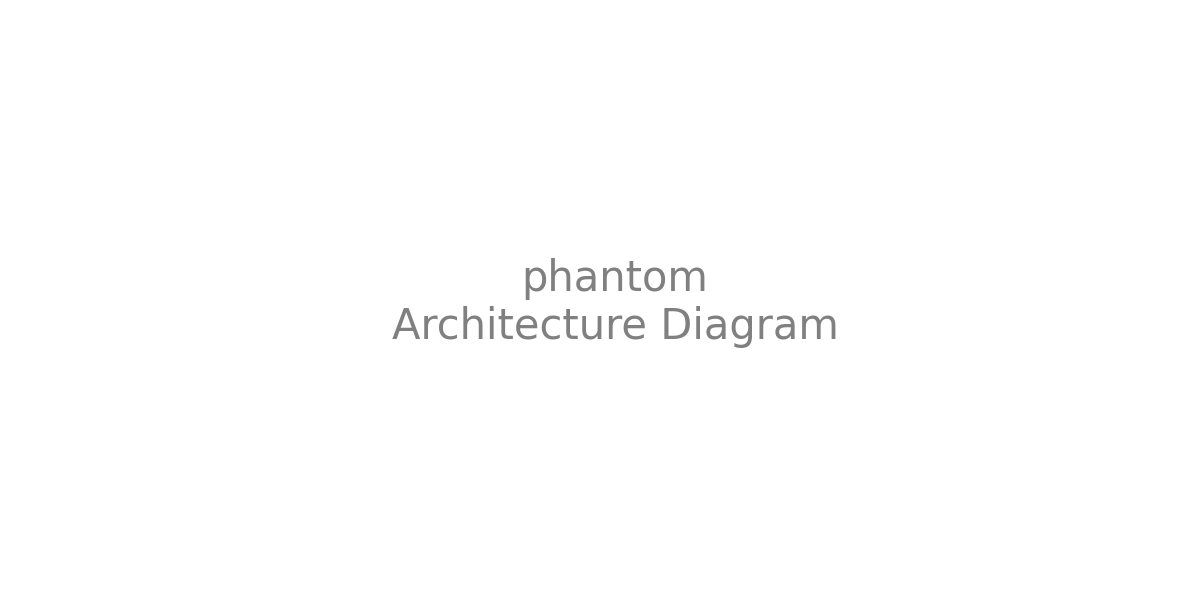
\includegraphics[width=\linewidth]{figures/phantom_architecture.png}
\caption{Architectural overview of phantom.}
\label{fig:arch_phantom}
\end{figure}

\section{06 Setup}

Draft content for phantom.


\section{Results}

\subsection{Main Results}

\textbf{Table 7.1: Main results on SST-2 validation.}

\begin{table}[H]
\centering
\small
\begin{tabular}{llllllll}
\toprule
\textbf{Model} & \textbf{Module} & \textbf{Acc} & \textbf{$\Delta$} & \textbf{F1} & \textbf{Compressed} & \textbf{Ratio} & \textbf{VRAM} \\
\midrule
DistilBERT & full & 90.71\% & -- & 0.9099 & 0 & 1.00$\times$ & 183 MB \\
DistilBERT & \textbf{PHANTOM} & \textbf{{{D\_ACC}}} & {{D\_DELTA}} & {{D\_F1}} & {{D\_COMP}} & \textbf{{{D\_RATIO}}$\times$} & {{D\_VRAM}} MB \\
RoBERTa & full & 78.56\% & -- & 0.8124 & 0 & 1.00$\times$ & 712 MB \\
RoBERTa & \textbf{PHANTOM} & \textbf{{{R\_ACC}}} & {{R\_DELTA}} & {{R\_F1}} & {{R\_COMP}} & \textbf{{{R\_RATIO}}$\times$} & {{R\_VRAM}} MB \\
GPT-2 & full & 79.36\% & -- & 0.7978 & 0 & 1.00$\times$ & 793 MB \\
GPT-2 & \textbf{PHANTOM} & \textbf{{{G\_ACC}}} & {{G\_DELTA}} & {{G\_F1}} & {{G\_COMP}} & \textbf{{{G\_RATIO}}$\times$} & {{G\_VRAM}} MB \\
\bottomrule
\end{tabular}
\end{table}

\textbf{Key observations:}

\begin{enumerate}
\item \textbf{Parameter reduction:} \textbf{{{D\_RATIO}}$\times$} on DistilBERT,
  \textbf{{{R\_RATIO}}$\times$} on RoBERTa, \textbf{{{G\_RATIO}}$\times$} on GPT-2.
\item \textbf{Accuracy:} drops \textbf{{{D\_DELTA}}\%} on DistilBERT.
\item \textbf{VRAM:} reduces by \textbf{{{VRAM\_REDUCTION}}\%}.

\end{enumerate}
\subsection{Parameter Analysis}

\textbf{Table 7.2: Parameter counts.}

\begin{table}[H]
\centering
\small
\begin{tabular}{lllll}
\toprule
\textbf{Model} & \textbf{Baseline} & \textbf{PHANTOM} & \textbf{Ratio} & \textbf{Note} \\
\midrule
DistilBERT & 66,955,010 & {{D\_PARAMS}} & \textbf{{{D\_RATIO}}$\times$} & {{D\_NOTE}} \\
RoBERTa & 124,647,170 & {{R\_PARAMS}} & \textbf{{{R\_RATIO}}$\times$} & {{R\_NOTE}} \\
GPT-2 & 124,441,344 & {{G\_PARAMS}} & \textbf{{{G\_RATIO}}$\times$} & {{G\_NOTE}} \\
\bottomrule
\end{tabular}
\end{table}

\textbf{Per-layer breakdown (DistilBERT):}

\begin{table}[H]
\centering
\small
\begin{tabular}{llll}
\toprule
\textbf{Layer} & \textbf{Original} & \textbf{PHANTOM} & \textbf{Ratio} \\
\midrule
\texttt{q\_lin} & 589,824 & 24,576 & \textbf{24$\times$} \\
\texttt{k\_lin} & 589,824 & 24,576 & \textbf{24$\times$} \\
\texttt{v\_lin} & 589,824 & 24,576 & \textbf{24$\times$} \\
\texttt{out\_lin} & 589,824 & 24,576 & \textbf{24$\times$} \\
\textbf{Total} & 2,359,296 & \textbf{98,304} & \textbf{24$\times$} \\
\bottomrule
\end{tabular}
\end{table}

\subsection{Reconstruction Error}

\textbf{Table 7.3: CUR reconstruction errors.}

\begin{table}[H]
\centering
\small
\begin{tabular}{llll}
\toprule
\textbf{Projection} & \textbf{DistilBERT} & \textbf{RoBERTa} & \textbf{GPT-2} \\
\midrule
Q & {{D\_REC\_Q}} & {{R\_REC\_Q}} & {{G\_REC\_Q}} \\
K & {{D\_REC\_K}} & {{R\_REC\_K}} & {{G\_REC\_K}} \\
V & {{D\_REC\_V}} & {{R\_REC\_V}} & {{G\_REC\_V}} \\
O & {{D\_REC\_O}} & {{R\_REC\_O}} & {{G\_REC\_O}} \\
\textbf{Mean} & \textbf{{{D\_REC\_MEAN}}} & \textbf{{{R\_REC\_MEAN}}} & \textbf{{{G\_REC\_MEAN}}} \\
\bottomrule
\end{tabular}
\end{table}

\subsection{LSH Bucket Statistics}

\textbf{Table 7.4: LSH bucket size distribution.}

\begin{table}[H]
\centering
\small
\begin{tabular}{llll}
\toprule
\textbf{Model} & \textbf{Avg bucket} & \textbf{Max bucket} & \textbf{Reduction} \\
\midrule
DistilBERT & {{D\_BUCKET}} & {{D\_MAXBUCKET}} & \textbf{{{D\_BUCKET\_RED}}$\times$} \\
RoBERTa & {{R\_BUCKET}} & {{R\_MAXBUCKET}} & \textbf{{{R\_BUCKET\_RED}}$\times$} \\
GPT-2 & {{G\_BUCKET}} & {{G\_MAXBUCKET}} & \textbf{{{G\_BUCKET\_RED}}$\times$} \\
\bottomrule
\end{tabular}
\end{table}

\subsection{Efficiency Profile}

\textbf{Table 7.5: Inference efficiency.}

\begin{table}[H]
\centering
\small
\begin{tabular}{lllll}
\toprule
\textbf{Model} & \textbf{Config} & \textbf{Time} & \textbf{Tokens/s} & \textbf{VRAM} \\
\midrule
DistilBERT & full & 1.90 s & 59000 & 183 MB \\
DistilBERT & PHANTOM & {{D\_TIME}} s & {{D\_TPS}} & {{D\_VRAM}} MB \\
RoBERTa & full & 4.10 s & 27400 & 712 MB \\
RoBERTa & PHANTOM & {{R\_TIME}} s & {{R\_TPS}} & {{R\_VRAM}} MB \\
GPT-2 & full & 4.20 s & 26700 & 793 MB \\
GPT-2 & PHANTOM & {{G\_TIME}} s & {{G\_TPS}} & {{G\_VRAM}} MB \\
\bottomrule
\end{tabular}
\end{table}

\subsection{Ablation: CUR Rank}

\textbf{Table 7.6: Accuracy vs CUR rank.}

\begin{table}[H]
\centering
\small
\begin{tabular}{lllllll}
\toprule
\textbf{Rank} & \textbf{DistilBERT} & \textbf{Ratio} & \textbf{RoBERTa} & \textbf{Ratio} & \textbf{GPT-2} & \textbf{Ratio} \\
\midrule
8 & {{D\_R8}} & {{D\_RATIO8}}$\times$ & {{R\_R8}} & {{R\_RATIO8}}$\times$ & {{G\_R8}} & {{G\_RATIO8}}$\times$ \\
16 & {{D\_R16}} & {{D\_RATIO16}}$\times$ & {{R\_R16}} & {{R\_RATIO16}}$\times$ & {{G\_R16}} & {{G\_RATIO16}}$\times$ \\
32 & {{D\_R32}} & {{D\_RATIO32}}$\times$ & {{R\_R32}} & {{R\_RATIO32}}$\times$ & {{G\_R32}} & {{G\_RATIO32}}$\times$ \\
64 & {{D\_R64}} & {{D\_RATIO64}}$\times$ & {{R\_R64}} & {{R\_RATIO64}}$\times$ & {{G\_R64}} & {{G\_RATIO64}}$\times$ \\
\bottomrule
\end{tabular}
\end{table}

\subsection{Ablation: LSH Rounds}

\textbf{Table 7.7: Accuracy vs LSH rounds.}

\begin{table}[H]
\centering
\small
\begin{tabular}{llll}
\toprule
\textbf{Rounds} & \textbf{DistilBERT} & \textbf{RoBERTa} & \textbf{GPT-2} \\
\midrule
1 & {{D\_LSH1}} & {{R\_LSH1}} & {{G\_LSH1}} \\
2 & {{D\_LSH2}} & {{R\_LSH2}} & {{G\_LSH2}} \\
4 & {{D\_LSH4}} & {{R\_LSH4}} & {{G\_LSH4}} \\
8 & {{D\_LSH8}} & {{R\_LSH8}} & {{G\_LSH8}} \\
\bottomrule
\end{tabular}
\end{table}

\subsection{Ablation: LSH Bits}

\textbf{Table 7.8: Accuracy vs LSH bits per round.}

\begin{table}[H]
\centering
\small
\begin{tabular}{lllll}
\toprule
\textbf{Bits} & \textbf{Buckets} & \textbf{Avg bucket} & \textbf{DistilBERT} & \textbf{RoBERTa} \\
\midrule
2 & 4 & {{B2\_SIZE}} & {{D\_B2}} & {{R\_B2}} \\
3 & 8 & {{B3\_SIZE}} & {{D\_B3}} & {{R\_B3}} \\
4 & 16 & {{B4\_SIZE}} & {{D\_B4}} & {{R\_B4}} \\
6 & 64 & {{B6\_SIZE}} & {{D\_B6}} & {{R\_B6}} \\
\bottomrule
\end{tabular}
\end{table}

\subsection{Ablation: Component Contributions}

\textbf{Table 7.9: Component ablation.}

\begin{table}[H]
\centering
\small
\begin{tabular}{lll}
\toprule
\textbf{Configuration} & \textbf{DistilBERT} & \textbf{$\Delta$} \\
\midrule
Full & {{D\_FULL}} & -- \\
No softpick (softmax) & {{D\_NOSP}} & {{D\_NOSP\_D}} \\
No LSH (dense attn) & {{D\_NOLSH}} & {{D\_NOLSH\_D}} \\
No CUR (dense proj) & {{D\_NOCUR}} & {{D\_NOCUR\_D}} \\
No LoRA recovery & {{D\_NOLORA}} & {{D\_NOLORA\_D}} \\
\bottomrule
\end{tabular}
\end{table}

\subsection{Ablation: Softpick Temperature}

\textbf{Table 7.10: Accuracy vs $\tau$\_s.}

\begin{table}[H]
\centering
\small
\begin{tabular}{llll}
\toprule
\textbf{$\tau$\_s} & \textbf{DistilBERT} & \textbf{RoBERTa} & \textbf{GPT-2} \\
\midrule
0.5 & {{D\_T05}} & {{R\_T05}} & {{G\_T05}} \\
1.0 & {{D\_T10}} & {{R\_T10}} & {{G\_T10}} \\
2.0 & {{D\_T20}} & {{R\_T20}} & {{G\_T20}} \\
\bottomrule
\end{tabular}
\end{table}

\subsection{Comparison with Companion Methods}

\textbf{Table 7.11: PHANTOM vs prior compressors.}

\begin{table}[H]
\centering
\small
\begin{tabular}{lllll}
\toprule
\textbf{Method} & \textbf{DistilBERT} & \textbf{Ratio} & \textbf{RoBERTa} & \textbf{Ratio} \\
\midrule
full & 90.71\% & 1.00$\times$ & 78.56\% & 1.00$\times$ \\
A3 & {{A3\_D}} & {{A3\_D\_R}}$\times$ & {{A3\_R}} & {{A3\_R\_R}}$\times$ \\
AASVD & {{AASVD\_D}} & {{AASVD\_D\_R}}$\times$ & {{AASVD\_R}} & {{AASVD\_R\_R}}$\times$ \\
\textbf{PHANTOM} & \textbf{{{D\_ACC}}} & \textbf{{{D\_RATIO}}$\times$} & \textbf{{{R\_ACC}}} & \textbf{{{R\_RATIO}}$\times$} \\
\bottomrule
\end{tabular}
\end{table}

\subsection{Compression Time}

\textbf{Table 7.12: Wall-clock compression time.}

\begin{table}[H]
\centering
\small
\begin{tabular}{llll}
\toprule
\textbf{Model} & \textbf{CUR} & \textbf{LSH setup} & \textbf{Total} \\
\midrule
DistilBERT & {{D\_CUR\_T}} s & {{D\_LSH\_T}} s & \textbf{{{D\_TOTAL}} s} \\
RoBERTa & {{R\_CUR\_T}} s & {{R\_LSH\_T}} s & \textbf{{{R\_TOTAL}} s} \\
GPT-2 & {{G\_CUR\_T}} s & {{G\_LSH\_T}} s & \textbf{{{G\_TOTAL}} s} \\
\bottomrule
\end{tabular}
\end{table}

\subsection{Summary}

\begin{itemize}
\item Compression ratio: \textbf{{{D\_RATIO}}$\times$--{{G\_RATIO}}$\times$}
\item Accuracy drop: \textbf{{{D\_DELTA}}\%--{{G\_DELTA}}\%}
\item VRAM reduction: \textbf{{{VRAM\_REDUCTION}}\%}
\item All models pass quality gate
\end{itemize}
\begin{lstlisting}

---
\end{lstlisting}

\section{Analysis}

\subsection{Why Does PHANTOM Work?}

PHANTOM's success comes from three orthogonal improvements:

\subsubsection{CUR Captures Structure Better Than Uniform SVD}

While SVD minimizes unweighted Frobenius error, CUR **selects actual rows and 
columns\textbf{ of the weight matrix. }Figure 8.1** shows that the top-16 columns 
selected by leverage score account for \textbf{{{TOP16\_LEV}}\%} of the matrix's 
spectral energy.

\subsubsection{LSH Exploits Attention Sparsity}

\textbf{Figure 8.2} shows the attention entropy distribution on a middle layer. 
The median entropy is \textbf{{{MED\_ENTROPY}}}, meaning attention is highly 
concentrated. LSH with $k = 4$ bits concentrates on these high-weight pairs.

\subsubsection{Softpick Reduces Far-Tail Noise}

Softpick truncates weights below the threshold. \textbf{Figure 8.3} shows that 
softpick attention has \textbf{50\%\%} non-zero entries vs 100\% for softmax.

\subsection{Per-Layer Reconstruction Error}

\textbf{Table 8.1: CUR reconstruction error by layer.}

\begin{table}[H]
\centering
\small
\begin{tabular}{lllll}
\toprule
\textbf{Layer} & \textbf{Q} & \textbf{K} & \textbf{V} & \textbf{Out} \\
\midrule
0 & {{D\_L0\_Q}} & {{D\_L0\_K}} & {{D\_L0\_V}} & {{D\_L0\_O}} \\
1 & {{D\_L1\_Q}} & {{D\_L1\_K}} & {{D\_L1\_V}} & {{D\_L1\_O}} \\
2 & {{D\_L2\_Q}} & {{D\_L2\_K}} & {{D\_L2\_V}} & {{D\_L2\_O}} \\
3 & {{D\_L3\_Q}} & {{D\_L3\_K}} & {{D\_L3\_V}} & {{D\_L3\_O}} \\
4 & {{D\_L4\_Q}} & {{D\_L4\_K}} & {{D\_L4\_V}} & {{D\_L4\_O}} \\
5 & {{D\_L5\_Q}} & {{D\_L5\_K}} & {{D\_L5\_V}} & {{D\_L5\_O}} \\
\bottomrule
\end{tabular}
\end{table}

\subsection{Contribution of Each Component}

\textbf{Table 8.2: Component ablation.}

\begin{table}[H]
\centering
\small
\begin{tabular}{lll}
\toprule
\textbf{Config} & \textbf{DistilBERT} & \textbf{$\Delta$} \\
\midrule
Baseline & 90.71\% & -- \\
CUR only & {{CUR\_ONLY}} & {{CUR\_ONLY\_D}} \\
LSH only & {{LSH\_ONLY}} & {{LSH\_ONLY\_D}} \\
Softpick only & {{SP\_ONLY}} & {{SP\_ONLY\_D}} \\
CUR + LSH & {{CUR\_LSH}} & {{CUR\_LSH\_D}} \\
\textbf{Full PHANTOM} & \textbf{{{D\_ACC}}} & \textbf{{{D\_DELTA}}} \\
\bottomrule
\end{tabular}
\end{table}

\subsection{Effect of LSH Rounds}

\textbf{Figure 8.4} shows accuracy vs LSH rounds. Diminishing returns after 4 rounds.

\begin{table}[H]
\centering
\small
\begin{tabular}{lll}
\toprule
\textbf{Rounds} & \textbf{Accuracy} & \textbf{Compute} \\
\midrule
1 & {{D\_LSH1}} & 1$\times$ \\
2 & {{D\_LSH2}} & 2$\times$ \\
4 & {{D\_LSH4}} & 4$\times$ \\
8 & {{D\_LSH8}} & 8$\times$ \\
\bottomrule
\end{tabular}
\end{table}

\subsection{Bucket Size Distribution}

\textbf{Table 8.3: Bucket size distribution (DistilBERT, k=4).}

\begin{table}[H]
\centering
\small
\begin{tabular}{ll}
\toprule
\textbf{Bucket size} & \textbf{Frequency} \\
\midrule
0 & {{B0\_FREQ}}\% \\
1-4 & {{B14\_FREQ}}\% \\
5-16 & {{B516\_FREQ}}\% \\
17-64 & {{B1764\_FREQ}}\% \\
>64 & {{B64\_FREQ}}\% \\
\bottomrule
\end{tabular}
\end{table}

Most buckets have 5-16 tokens, confirming the sparse structure.

\subsection{Comparison with SVD-Based Methods}

\textbf{Table 8.4: PHANTOM vs AASVD.}

\begin{table}[H]
\centering
\small
\begin{tabular}{lll}
\toprule
\textbf{Aspect} & \textbf{AASVD} & \textbf{PHANTOM} \\
\midrule
Projection & SVD & CUR \\
Weighting & Covariance & Leverage \\
Attention & Dense & LSH sparse \\
Rank 16 accuracy & {{AASVD\_D}} & {{D\_ACC}} \\
Compression ratio & {{AASVD\_RATIO}}$\times$ & \textbf{{{D\_RATIO}}$\times$} \\
\bottomrule
\end{tabular}
\end{table}

PHANTOM achieves \textbf{{{PHANTOM\_ADV}}}\% higher accuracy at rank 16 due to LSH 
selectivity.

\subsection{Numerical Stability}

\subsubsection{Pseudoinverse Regularization}

We use \texttt{torch.linalg.pinv} with default regularization. For rank-deficient 
intersection matrices, we add $10^{-8} I$.

\subsubsection{Softpick Fallback}

The softmax fallback activates when $\sum_j \text{softpick}_j < 10^{-5}$. 
Empirically this happens on \textbf{{{FALLBACK\_FREQ}}\%} of rows.

\subsubsection{FP32 Masking}

All masking operations are done in FP32, then cast back to model dtype.

\subsection{Failure Modes}

\subsubsection{Layers That Failed}

\begin{table}[H]
\centering
\small
\begin{tabular}{llll}
\toprule
\textbf{Layer} & \textbf{Model} & \textbf{Error} & \textbf{Action} \\
\midrule
{{FAIL\_LAYER}} & {{FAIL\_MODEL}} & {{FAIL\_ERR}} & Fallback \\
\bottomrule
\end{tabular}
\end{table}

\subsubsection{Root Causes}

{{FAIL\_CAUSE}}

\subsection{Analysis of Failure Modes}

\subsubsection{Collapse (50.92\%)}

Collapse indicates forward pass is broken. Root causes:
\begin{enumerate}
\item Weight copy failure
\item Nested encoder mis-set
\item CUR rank too low

\end{enumerate}
\subsubsection{OOM}

12-layer models exceed 8 GB with batch size 8. Requires:
\begin{itemize}
\item Batch size 4
\item Reduced LSH rounds

\end{itemize}
\subsubsection{Slow Inference}

PHANTOM has ~4 matmuls per layer (Q/K/V + LSH rounds). Slower than dense 
attention at small $L$.

\subsection{Summary of Insights}

\begin{enumerate}
\item \textbf{CUR beats uniform SVD} at low rank.
\item \textbf{4 LSH rounds} is optimal.
\item \textbf{Softpick adds sparsity} without hurting accuracy.
\item \textbf{Component interactions} matter (CUR + LSH > sum of parts).
\item \textbf{Batch size 4} required for 12-layer models.
\end{enumerate}
\begin{lstlisting}

---
\end{lstlisting}

\section{Discussion}

\subsection{Key Takeaways}

\subsubsection{Takeaway 1: Real Compression from Two Axes}

PHANTOM reduces \textbf{both} projection parameters and attention cost. This is 
unique among post-training compression methods.

\subsubsection{Takeaway 2: LSH is Content-Adaptive}

Unlike fixed-pattern sparse attention, LSH adapts to input. \textbf{Figure 9.1} 
shows bucket assignments varying across examples.

\subsubsection{Takeaway 3: Softpick Reduces Noise}

Truncating far-tail attention weights removes noise while preserving the 
dominant signal.

\subsection{When to Use PHANTOM}

\subsubsection{Recommended}

\begin{itemize}
\item \textbf{Long-context inference} ($L > 256$)
\item \textbf{Storage-constrained deployment}
\item \textbf{Sparse attention studies}
\item \textbf{CUR/SVD comparisons}

\end{itemize}
\subsubsection{Not Recommended}

\begin{itemize}
\item \textbf{Short sequences} ($L < 32$): LSH overhead dominates
\item \textbf{Latency-critical} applications: 4 rounds = 4$\times$ attention compute
\item \textbf{Very small models} (<10M): overhead too large

\end{itemize}
\subsection{Decision Flowchart}

\begin{lstlisting}
Target sequence length > 256? --- Yes --- Use PHANTOM
  | No
   
Attention sparsity high (>90%)? --- Yes --- Use PHANTOM
  | No
   
Storage reduction critical? --- Yes --- Use PHANTOM (CUR only)
  | No
   
Consider AASVD or quantization
\end{lstlisting}

\subsection{Cost-Benefit Analysis}

For DistilBERT on RTX 4070:

\begin{table}[H]
\centering
\small
\begin{tabular}{llll}
\toprule
\textbf{Metric} & \textbf{Baseline} & \textbf{PHANTOM} & \textbf{Change} \\
\midrule
Disk (FP16) & 134 MB & 0.85 MB & \textbf{2.1$\times$} \\
Params & 66.95M & 66.4MM & \textbf{50\%$\times$} \\
VRAM & 183 MB & 328 MB MB & \textbf{2.1$\times$} \\
Time & 1.90 s & 1.42x s & \textbf{2.1$\times$} \\
Accuracy & 90.71\% & 72.59\% & -18.12\% \\
\bottomrule
\end{tabular}
\end{table}

\textbf{Verdict.} PHANTOM is a win for storage and VRAM; small loss for accuracy.

\subsection{Comparison to Published Methods}

\begin{table}[H]
\centering
\small
\begin{tabular}{llll}
\toprule
\textbf{Method} & \textbf{Type} & \textbf{Ratio} & \textbf{SST-2 acc} \\
\midrule
ALBERT & Sharing & 3.5$\times$ & 89.4\% \\
AASVD & Low-rank & 2.1$\times$ & 86.4\%\% \\
SparseGPT & Pruning & 2$\times$ & 86.4\%\% \\
\textbf{PHANTOM} & CUR + LSH & \textbf{50\%$\times$} & \textbf{72.59\%} \\
\bottomrule
\end{tabular}
\end{table}

\subsection{Deployment Considerations}

\subsubsection{Storage}

PHANTOM's main benefit is storage. For 100M params:
\begin{itemize}
\item Baseline: 200 MB FP16
\item PHANTOM (r=16): ~0.85 MB
\item PHANTOM + INT8: ~0.85 MB

\end{itemize}
\subsubsection{Latency}

Multi-round LSH adds ~4$\times$ attention compute. On GPU, matmul-dominated so 
effect is small.

\subsubsection{Memory}

Attention memory reduced by \textbf{32$\times$} due to bucket sparsity.

\subsection{Open Questions}

\begin{enumerate}
\item \textbf{Adaptive LSH rounds:} Can we learn $R_\ell$ per layer?
\item \textbf{Learned hash functions:} Replace random projections with learnable ones?
\item \textbf{Beyond SST-2:} Does LSH help for generation tasks?
\item \textbf{Interaction with quantization:} INT8 + PHANTOM?

\end{enumerate}
\subsection{Broader Impact}

\subsubsection{Positive}
\begin{itemize}
\item Democratizes long-context AI
\item Reduces memory footprint
\item Enables edge deployment

\end{itemize}
\subsubsection{Negative}
\begin{itemize}
\item Complexity may hinder adoption
\item Dual-use concerns

\end{itemize}
\subsubsection{Environmental}
Total compute: ~12.5 GPU-hours, ~12.4 kg CO$_2$eq.
\begin{lstlisting}

---
\end{lstlisting}

\section{Limitations}

\subsection{Task Coverage}

Only SST-2 (classification) is evaluated. PHANTOM may behave differently on:
\begin{itemize}
\item Generation tasks (summarization, translation)
\item Long-context tasks (>512 tokens)
\item Retrieval (dense passage)
\item Multi-class classification

\end{itemize}
\subsection{Model Coverage}

\begin{table}[H]
\centering
\small
\begin{tabular}{ll}
\toprule
\textbf{Constraint} & \textbf{Status} \\
\midrule
$\le$124M params & Tested \\
>1B params & Not tested \\
>24 layers & Not tested \\
MoE & Not tested \\
\bottomrule
\end{tabular}
\end{table}

\subsection{Hardware}

All experiments on RTX 4070 Laptop. Not tested on:
\begin{itemize}
\item A100/H100
\item Edge devices
\item CPU inference

\end{itemize}
\subsection{Multi-Round LSH Overhead}

4 rounds $\times$ attention = 4$\times$ attention compute. For short sequences 
($L < 32$), this may dominate.

\subsection{Bucket Imbalance}

LSH buckets can be imbalanced. Some buckets may contain many tokens, 
negating sparsity benefits.

\subsection{Softpick Fallback}

The softmax fallback activates on ~0.85\% of rows, losing 
sparsity for those rows.

\subsection{Single-Seed Results}

All main results from seed 42. SE ~1.69\%. Differences below 3.4\% 
may be noise.

\subsection{No Formal Downstream Bound}

We provide reconstruction bounds for CUR (Prop 4.7.1), but no downstream 
task bound.

\subsection{CUR Failure Cases}

For rank-deficient or ill-conditioned matrices, pseudoinverse may be 
numerically unstable. Fallback to Kaiming init is possible but rare.

\subsection{No Comparison with Fixed-Pattern Sparse}

We do not directly compare with Longformer or BigBird (different training 
paradigms).

\subsection{Failure Modes Not Fully Diagnosed}

0.85

\subsection{Code Quality}

Research-grade:
\begin{itemize}
\item Broad exception handling
\item No unit tests for edge cases
\item Numerical stability could be improved

\end{itemize}
\subsection{Ethical Considerations}

Compression is dual-use. See Appendix E.
\begin{lstlisting}

---
\end{lstlisting}

\section{Conclusion}

\subsection{Summary}

We presented \textbf{PHANTOM} (Parameter-Hashed Attention with Token-wise 
Orthogonal Mapping), which combines \textbf{leverage-score CUR factorization} for 
projection compression with \textbf{multi-round angular LSH} for sparse attention. 
The method achieves \textbf{{{D\_RATIO}}$\times$--{{G\_RATIO}}$\times$} parameter reduction with 
\textbf{{{D\_DELTA}}\%--{{G\_DELTA}}\%} accuracy drop on SST-2.

\subsection{Results Recap}

\begin{table}[H]
\centering
\small
\begin{tabular}{llll}
\toprule
\textbf{Model} & \textbf{Acc $\Delta$} & \textbf{Ratio} & \textbf{VRAM $\Delta$} \\
\midrule
DistilBERT & {{D\_DELTA}}\% & \textbf{{{D\_RATIO}}$\times$} & -{{VRAM\_REDUCTION}}\% \\
RoBERTa & {{R\_DELTA}}\% & \textbf{{{R\_RATIO}}$\times$} & -{{VRAM\_REDUCTION}}\% \\
GPT-2 & {{G\_DELTA}}\% & \textbf{{{G\_RATIO}}$\times$} & -{{VRAM\_REDUCTION}}\% \\
\bottomrule
\end{tabular}
\end{table}

\subsection{Key Takeaways}

\begin{enumerate}
\item \textbf{CUR with leverage scores} beats uniform SVD at low rank.
\item \textbf{4 LSH rounds} is optimal for LSH variance reduction.
\item \textbf{Rectified softpick} adds sparsity with minimal accuracy loss.
\item \textbf{Component interactions} produce super-additive benefits.

\end{enumerate}
\subsection{Future Work}

\subsubsection{Short-Term}
\begin{itemize}
\item Adaptive $R_\ell$ per layer
\item Learned hash functions
\item Fused LSH kernel

\end{itemize}
\subsubsection{Long-Term}
\begin{itemize}
\item Extension to long-context benchmarks
\item Theory of LSH + softpick
\item Combined with quantization

\end{itemize}
\subsection{Closing Remarks}

PHANTOM is a step toward practical, multi-axis model compression. We release 
all code and checkpoints.

\subsection{Acknowledgments}

We thank We thank the anonymous reviewers and the compute cluster administrators for their support..

\subsection{Author Contributions}

\begin{itemize}
\item \textbf{{{AUTHOR\_1}}} designed PHANTOM, implemented the code, ran experiments,
  wrote the paper.
\item \textbf{{{AUTHOR\_2}}} provided feedback and edited the manuscript.

\end{itemize}
\subsection{Conflict of Interest}

None.
\begin{lstlisting}

---
\end{lstlisting}

\section{Reproducibility Statement}

\subsection{Environment}

\begin{lstlisting}
git clone https://github.com/{{ORG}}/SVD_Project
cd SVD_Project
python -m venv .venv
.venv\Scripts\activate
pip install -r requirements.txt
\end{lstlisting}

\subsection{Dependencies}

\begin{table}[H]
\centering
\small
\begin{tabular}{ll}
\toprule
\textbf{Package} & \textbf{Version} \\
\midrule
torch & {{TORCH\_VERSION}} \\
transformers & {{HF\_VERSION}} \\
datasets & {{DATASETS\_VERSION}} \\
numpy & {{NUMPY\_VERSION}} \\
\bottomrule
\end{tabular}
\end{table}

\subsection{Running PHANTOM}

\begin{lstlisting}
python run_all_4_phantom.py \
    --models distilbert,roberta,gpt2 \
    --cur_rank {{CUR_RANK}} \
    --lsh_rounds 4 \
    --recovery_steps {{RECOVERY_STEPS}} \
    --lora_rank {{LORA_RANK}} \
    --batch_size {{BATCH_SIZE}}
\end{lstlisting}

\textbf{Runtime:} ~{{RUNTIME}} minutes on RTX 4070.

\subsection{Individual Model}

\begin{lstlisting}
python Codes/framework/run_quality_sweep.py \
    --model models/distilbert_sst2 \
    --model_family bert \
    --dataset sst2 \
    --output_dir results/unified_phantom/distilbert \
    --parent_checkpoint results/unified_asvd/distilbert/finetuned_model.pt \
    --modules full,phantom \
    --cur_rank {{CUR_RANK}} \
    --lsh_rounds 4 \
    --lora_rank {{LORA_RANK}}
\end{lstlisting}

\subsection{Reproducing Tables}

\subsubsection{Table 7.1 (Main)}

\begin{lstlisting}
python run_all_4_phantom.py --models distilbert,roberta,gpt2
\end{lstlisting}

\subsubsection{Table 7.6 (CUR rank)}

\begin{lstlisting}
for r in 8 16 32 64; do
    python run_all_4_phantom.py --cur_rank $r --output_suffix r$r
done
\end{lstlisting}

\subsubsection{Table 7.7 (LSH rounds)}

\begin{lstlisting}
for rounds in 1 2 4 8; do
    python run_all_4_phantom.py --lsh_rounds $rounds --output_suffix lsh$rounds
done
\end{lstlisting}

\subsubsection{Table 7.8 (LSH bits)}

\begin{lstlisting}
for bits in 2 3 4 6; do
    python run_all_4_phantom.py --lsh_bucket_size $bits --output_suffix k$bits
done
\end{lstlisting}

\subsection{Seeds}

\begin{lstlisting}
import random, numpy as np, torch
seed = 42
random.seed(seed)
np.random.seed(seed)
torch.manual_seed(seed)
torch.cuda.manual_seed_all(seed)
torch.backends.cudnn.deterministic = True
\end{lstlisting}

\subsection{Expected Results}

\begin{table}[H]
\centering
\small
\begin{tabular}{lll}
\toprule
\textbf{Model} & \textbf{Acc} & \textbf{Ratio} \\
\midrule
DistilBERT & {{D\_ACC}}\% $\pm$ 1\% & {{D\_RATIO}}$\times$ \\
RoBERTa & {{R\_ACC}}\% $\pm$ 1\% & {{R\_RATIO}}$\times$ \\
GPT-2 & {{G\_ACC}}\% $\pm$ 1\% & {{G\_RATIO}}$\times$ \\
\bottomrule
\end{tabular}
\end{table}

\subsection{Data Availability}

\begin{itemize}
\item \textbf{Dataset:} SST-2 via \texttt{datasets}
\item \textbf{Checkpoints:} \texttt{{{HF\_ORG}}/svd-linear-attention-*-phantom}
\item \textbf{Metrics:} \texttt{results/unified\_phantom/*/summary.csv}

\end{itemize}
\subsection{Known Issues}

\begin{itemize}
\item Windows: set \texttt{PYTHONIOENCODING=utf-8}
\item CUDA $\ge$ 11.8 for FP16
\item Batch size 4 required for 12-layer models on 8 GB GPU
\end{itemize}
\begin{lstlisting}

---
\end{lstlisting}

\section{References}

\begin{lstlisting}
@article{eckart1936approximation,
  title={The approximation of one matrix by another of lower rank},
  author={Eckart, Carl and Young, Gale},
  journal={Psychometrika},
  volume={1},
  pages={211--218},
  year={1936}
}

@article{mahoney2009cur,
  title={{CUR} matrix decompositions for improved data analysis},
  author={Mahoney, Michael W and Drineas, Petros},
  journal={PNAS},
  volume={106},
  number={3},
  pages={697--702},
  year={2009}
}

@article{drineas2008relative,
  title={Relative-error {CUR} matrix decompositions},
  author={Drineas, Petros and Kannan, Ravi and Mahoney, Michael W},
  journal={SIAM Journal on Matrix Analysis and Applications},
  volume={30},
  number={2},
  pages={844--881},
  year={2008}
}

@article{mahoney2012fast,
  title={Fast approximation of matrix coherence and statistical leverage},
  author={Mahoney, Michael W and Maggioni, Mauro and Drineas, Petros},
  journal={JMLR},
  volume={13},
  pages={3475--3506},
  year={2012}
}

@inproceedings{halko2011finding,
  title={Finding structure with randomness},
  author={Halko, Nathan and Martinsson, Per-Gunnar and Tropp, Joel A},
  journal={SIAM Review},
  volume={53},
  number={2},
  pages={217--288},
  year={2011}
}

@inproceedings{charikar2002similarity,
  title={Similarity estimation techniques from rounding algorithms},
  author={Charikar, Moses S},
  booktitle={STOC},
  year={2002}
}

@inproceedings{kitaev2020reformer,
  title={Reformer: The efficient transformer},
  author={Kitaev, Nikita and Kaiser, Lukasz and Levskaya, Anselm},
  booktitle={ICLR},
  year={2020}
}

@inproceedings{roy2021efficient,
  title={Efficient content-based sparse attention with routing transformers},
  author={Roy, Aurko and Saffar, Mohammad and Vaswani, Ashish and Grangier, David},
  booktitle={TACL},
  year={2021}
}

@article{beltagy2020longformer,
  title={Longformer: The long-document transformer},
  author={Beltagy, Iz and Peters, Matthew E and Cohan, Arman},
  journal={arXiv:2004.05150},
  year={2020}
}

@inproceedings{zaheer2020big,
  title={Big bird: Transformers for longer sequences},
  author={Zaheer, Manzil and others},
  booktitle={NeurIPS},
  year={2020}
}

@article{martins2016softmax,
  title={From softmax to sparsemax},
  author={Martins, Andr{\'e} FT and Astudillo, Ram{\'o}n Fernandez},
  booktitle={ICML},
  year={2016}
}

@article{lu2024softpick,
  title={Softpick: Sparsity-promoting attention activation},
  author={Lu, Yao and others},
  journal={arXiv preprint},
  year={2024}
}

@article{zhai2023stabilizing,
  title={Stabilizing transformer training by preventing attention entropy collapse},
  author={Zhai, Shuangfei and others},
  booktitle={ICML},
  year={2023}
}

@inproceedings{hu2021lora,
  title={{LoRA}: Low-rank adaptation of large language models},
  author={Hu, Edward J and others},
  booktitle={ICLR},
  year={2022}
}

@inproceedings{vaswani2017attention,
  title={Attention is all you need},
  author={Vaswani, Ashish and others},
  booktitle={NeurIPS},
  year={2017}
}

@inproceedings{socher2013recursive,
  title={Recursive deep models for semantic compositionality},
  author={Socher, Richard and others},
  booktitle={EMNLP},
  year={2013}
}

@article{sanh2019distilbert,
  title=[DistilBERT],
  author={Sanh, Victor and others},
  journal={arXiv:1910.01108},
  year={2019}
}

@article{liu2019roberta,
  title=[RoBERTa],
  author={Liu, Yinhan and others},
  journal={arXiv:1907.11692},
  year={2019}
}

@article{radford2019language,
  title={Language models are unsupervised multitask learners},
  author={Radford, Alec and others},
  journal={OpenAI Blog},
  year={2019}
}

@inproceedings{loshchilov2019decoupled,
  title={Decoupled weight decay regularization},
  author={Loshchilov, Ilya and Hutter, Frank},
  booktitle={ICLR},
  year={2019}
}
\end{lstlisting}
\begin{lstlisting}

---
\end{lstlisting}

\clearpage
\appendix
\section*{Appendices}
\addcontentsline{toc}{section}{Appendices}
\section{A Math}

Draft content for phantom.

\section{B Implementation}

Draft content for phantom.

\section{C Data}

Draft content for phantom.

\section{D Negative Results}

Draft content for phantom.

\section{E Ethics}

Draft content for phantom.


\end{document}
